\documentclass[12pt, twoside]{article}
\usepackage[letterpaper, margin=1in, headsep=0.5in]{geometry}
\usepackage[english]{babel}
\usepackage[utf8]{inputenc}
\usepackage{amsmath}
\usepackage{amsfonts}
\usepackage{amssymb}
\usepackage{tikz}
%\usetikzlibrary{quotes, angles}

\usepackage{graphicx}
\usepackage{enumitem}
\usepackage{multicol}

\usepackage{fancyhdr}
\pagestyle{fancy}
\fancyhf{}
\renewcommand{\headrulewidth}{0pt} % disable the underline of the header

\fancyhead[LE]{\thepage}
\fancyhead[RO]{\thepage \\ Name: \hspace{4cm} \,\\}
\fancyhead[LO]{BECA / Dr. Huson / Geometry\\* Unit 9: Congruence \& similarity transformations\\* 2 March 2020}

\begin{document}
\subsubsection*{9.7 Classwork: Similarity ratios, dilation, transformations, symmetry}
\begin{enumerate}

\item Find the image of $P(1,-4)$ after the translation $(x,y) \rightarrow (x-5,y+4)$. \vspace{2cm}
  
\item Given $\triangle ABC \sim \triangle DEF$. $m\angle A = 90^\circ$ and $m\angle F = 45^\circ$. Find the measure of $\angle D$. \vspace{2cm}

\item In the diagram of $\triangle ABC$, $D$ is a point on $\overline{BA}$, $E$ is a point on $\overline{BC}$, and $\overline{DE}$ is drawn. \\*[2pt] 
  If $BD=6.5$, $DA=13$, and $BE=8$, what is the length of $\overline{BC}$ so that $\overline{AC} \parallel \overline{DE}$?
  \begin{flushright}
      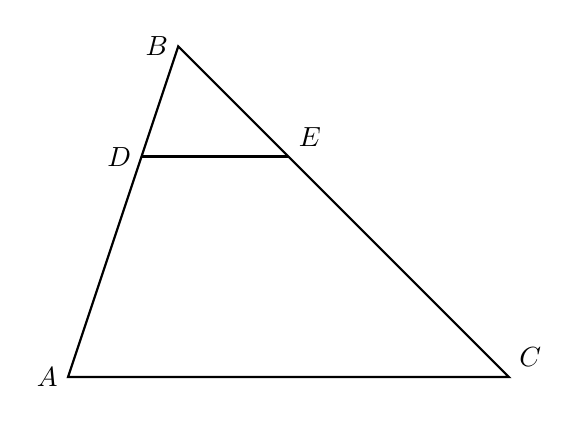
\begin{tikzpicture}[scale=0.7]
        \draw [thick]
        (0,0)node[left]{$A$}--
        (8,0)node[above right]{$C$}--
        (2,6)node[left]{$B$}--cycle;
        \draw [thick]
        (4/3,4)node[left]{$D$}--
        (4,4)node[above right]{$E$};
      \end{tikzpicture}
    \end{flushright}

\item In diagram below, each centimeter represents one foot. Find the length of each side in feet. (measure with a metric scale)
  \begin{multicols}{2}
    \begin{enumerate}[itemsep=1.5cm]
      \item $AC=$
      \item $BC=$
      \item $AB=$ 
      \item Find the area of $\triangle ABC$
    \end{enumerate}
  \begin{center}
    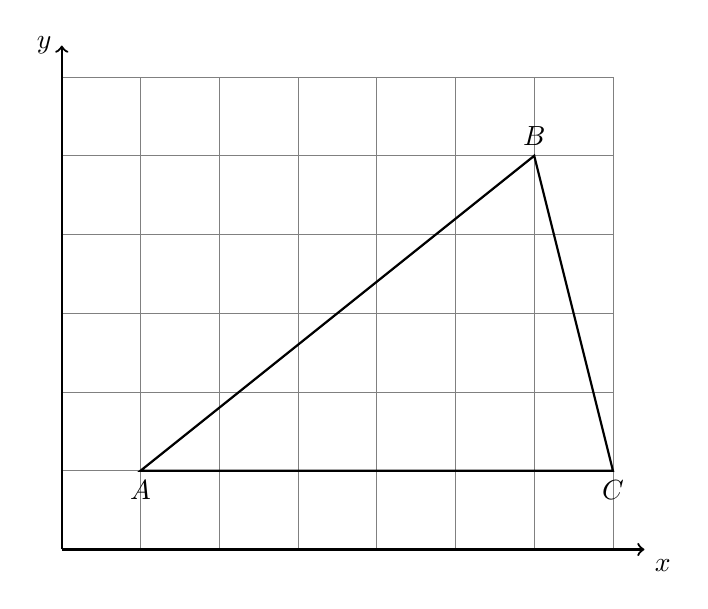
\begin{tikzpicture}
      \draw [help lines] (0,0) grid (7,6);
      \draw [thick, ->] (0,0) -- (7.4,0) node [below right] {$x$};
      \draw [thick, ->] (0,0)--(0,6.4) node [left] {$y$};
      \draw [thick] (1,1)node[below]{$A$}--(7,1)node[below]{$C$}
      --(6,5)node[above]{$B$}--cycle;
    \end{tikzpicture}
  \end{center}
\end{multicols}%\vspace{2cm}

\newpage
\item Given $\triangle ABP \sim \triangle JKP$ as shown below. $AB=13.5$, $AP=10.0$, $BP=9$, and $JP=27.0$. Find $JK$.
  \begin{flushright}
  \begin{tikzpicture}[scale=1.4]
      \draw [thick]
        (-0.25,-1)node[below left]{$B$}--
        (0.5,2)node[left]{$K$}--
        (4,0)node[below left]{$J$}--
        (0,0)node[above left]{$P$}--
        (-2,0)node[left]{$A$}--cycle;
    \end{tikzpicture}
    \end{flushright}
    \vspace{0.5cm}

\item A dilation centered at the origin with scale factor $k=\frac{1}{2}$ maps $\overline{AB} \rightarrow \overline{A'B'}$. 
  \begin{multicols}{2}
    \begin{enumerate}
      \item Draw and label the image.
      \item What is the ratio of the length of $\overline{A'B'}$ to $\overline{AB}$?
      \item What is the relationship of the slope of $\overline{A'B'}$ and $\overline{AB}$?
      \begin{flushright}
        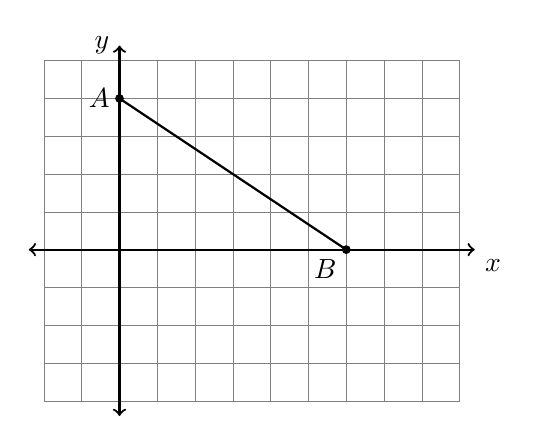
\begin{tikzpicture}[scale=.48]
          \draw [help lines] (-2,-4) grid (9,5);
          \draw [thick, <->] (-2.4,0) -- (9.4,0) node [below right] {$x$};
          \draw [thick, <->] (0,-4.4)--(0,5.4) node [left] {$y$};
          \draw [thick] (0,4)--(6,0);
          \draw [fill] (0,4) circle [radius=0.1] node[left] {$A$};
          \draw [fill] (6,0) circle [radius=0.1] node[below left] {$B$};
        \end{tikzpicture}
      \end{flushright}
    \end{enumerate}
    \end{multicols} \vspace{2cm}

\item A translation maps $N(-2, 7) \rightarrow N'(-4,9)$. What is the image of $M(3,-1)$ under the same translation?
      
\newpage
\item The vertices of $\triangle JKL$ have the coordinates $J(-4,-2)$, $K(4,2)$, and $L(-2,4)$, as shown. \\[0.25cm]
  Apply a dilation to $\triangle JKL \rightarrow \triangle J'K'L'$, centered on the origin and with a scale factor $k=1.5$. Draw the image $\triangle J'K'L'$ on the set of axes below, labeling the vertices, and make a table showing the correspondence of both triangles' coordinate pairs.
    \begin{flushright}
      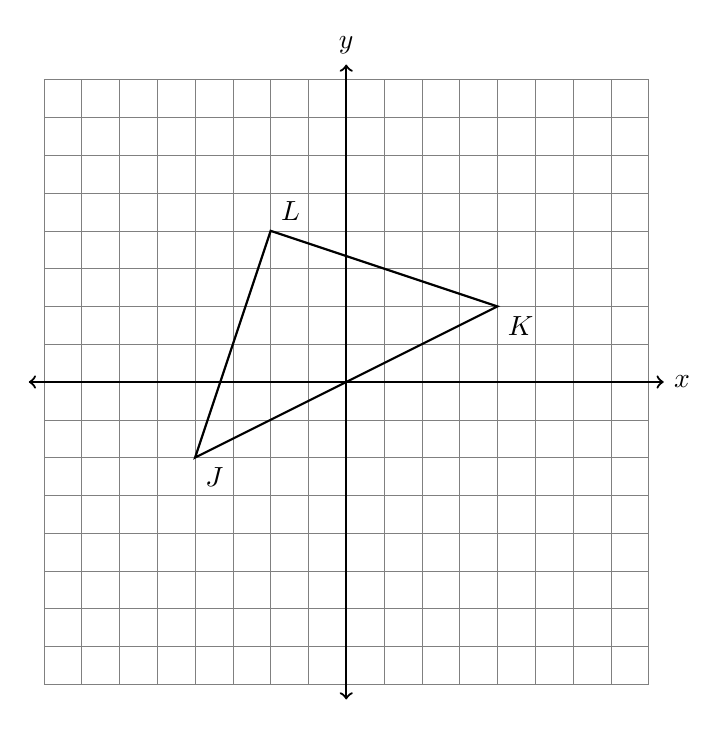
\begin{tikzpicture}[scale=.48]
        \draw [help lines] (-8,-8) grid (8,8);
        \draw [thick, <->] (-8.4,0) -- (8.4,0) node [right] {$x$};
        \draw [thick, <->] (0,-8.4)--(0,8.4) node [above] {$y$};
        \draw [thick]
          (-4,-2) node[below right] {$J$}--
          (4,2) node[below right] {$K$}--
          (-2,4) node[above right] {$L$}--
          cycle;
      \end{tikzpicture}
    \end{flushright}
    
\item A dilation centered at $A$ maps $\triangle ABC \rightarrow \triangle ADE$. Given $AB = 9$, $AC = 6$, $BD = 15$, and $DE = 16$. Find  $AD$ and the scale factor $k$. Then find $AE$ and $BC$. %\vspace{1cm}
  \begin{multicols}{2}
    \begin{enumerate}
      \item $AD=$ \vspace{0.3cm}
      \item $k=$ \vspace{0.3cm}
      \item $AE=$ \vspace{0.3cm}
      \item $BC=$
    \end{enumerate}
    \begin{flushright}
      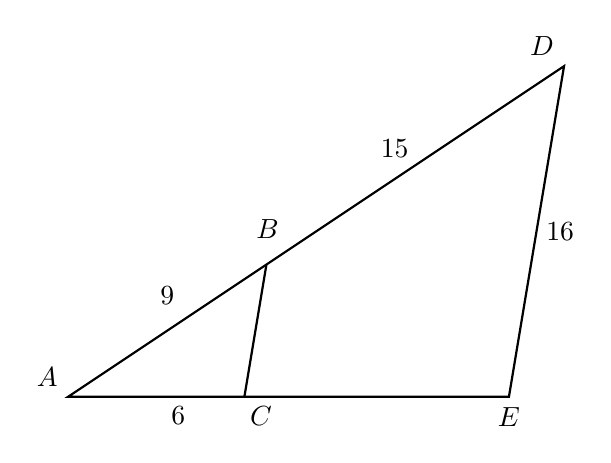
\begin{tikzpicture}[scale=0.7]
        \draw [-, thick] (0,0) node[above left]{$A$}--
        (8,0) node[below]{$E$}--
        (9,6) node[above left]{$D$}--cycle;
        \draw [thick] (3.2,0)--(3.6,2.4);
        \node at (3.5,0) [below]{$C$};
        \node at (4,2.7) [above left]{$B$};
        \node at (2, 0) [below]{$6$};
        \node at (1.8,1.5) [above]{$9$};
        \node at (8.5, 3) [right]{$16$};
        \node at (5.5, 4.5) [right]{$15$}; \vspace{1cm}
      \end{tikzpicture}
    \end{flushright} 
  \end{multicols}\vspace{1cm}

\newpage
\item The line $\overleftrightarrow{AB}$ has the equation $y=-\frac{1}{2}x+2$. Apply a dilation mapping $\overleftrightarrow{AB} \rightarrow \overleftrightarrow{A'B'}$ with a factor of $k=2$ centered at the origin. Draw and label the image on the grid. Write the equation of the line $\overleftrightarrow{A'B'}$.
  \begin{flushright} %4 quadrant regents grid w T-Chart
  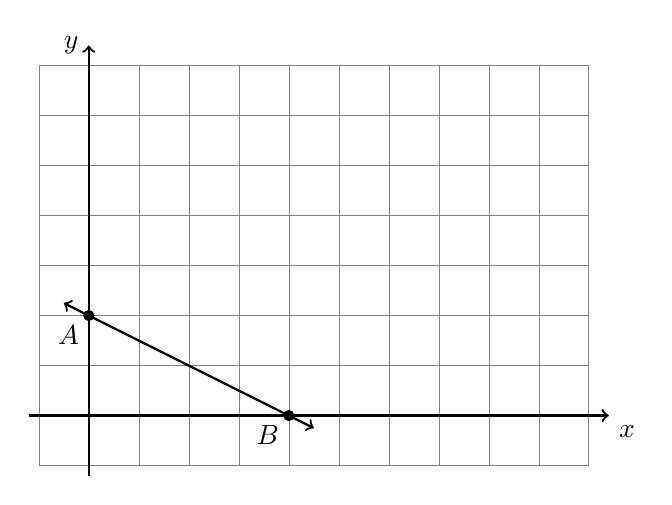
\begin{tikzpicture}[scale=.635]
    \draw [help lines] (-1,-1) grid (10,7);
    \draw [thick, ->] (-1.2,0) -- (10.4,0) node [below right] {$x$};
    \draw [thick, ->] (0,-1.2)--(0,7.4) node [left] {$y$};
    \draw [<->, thick] (-0.5,2.25)--(4.5,-0.25);
    \draw [fill] (0,2) circle [radius=0.1]node[below left]{$A$};
    %\draw [fill] (3,0) circle [radius=0.1]node[below left]{$C$};
    \draw [fill] (4,0) circle [radius=0.1]node[below left]{$B$};
  \end{tikzpicture}
  \end{flushright}

\item The diagram below shows $\triangle ABC$, with $\overline{AEB}$, $\overline{ADC}$, and $\angle ACB \cong \angle AED$. $AB=18$, $AD=12$, $AE=9$, and $DE=7$. Find the scale factor $k$, $AC$, and $BC$.
  \begin{multicols}{2}
  \begin{enumerate}
    \item $k=$ \vspace{1cm}
    \item $AC=$ \vspace{1cm}
    \item $BC=$  \vspace{1cm}
  \end{enumerate}
    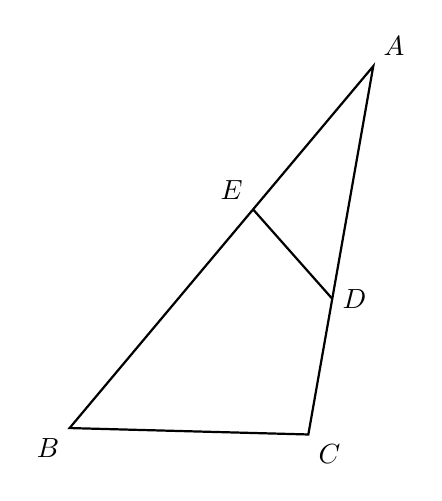
\begin{tikzpicture}[scale=1.0]
      \draw [thick]
      (0,0) node[above right] {$A$}--
      (230:6) node[below left] {$B$}--
      (260:4.75) node[below right] {$C$}--cycle;
      \draw [thick]
      (230:2.375) node[above left] {$E$}--
      (260:3) node[right] {$D$}--cycle;
    \end{tikzpicture}
  \end{multicols}\vspace{0.5cm}

\item In the diagram below, the chords $\overline{AE}$ and $\overline{BD}$ intersect at $C$. Given $\triangle ABC \sim \triangle DEC$, $BC=6$, $CD=10$, and $CE=8$. Determine the length of $\overline{CA}$.
  \begin{flushright}
  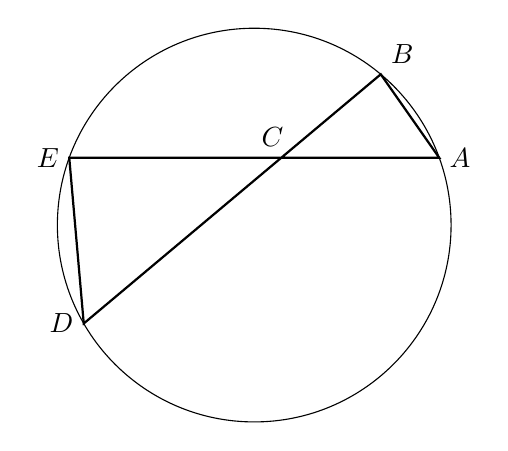
\begin{tikzpicture}[scale=.5]
    \draw (0,0) circle[radius=5];
    \draw [thick]
    (20:5) node[right] {$A$}--
    (160:5) node[left] {$E$}--
    (210:5) node[left] {$D$}--
    (50:5) node[above right] {$B$}--cycle;
    \draw (75:1.8) node[above] {$C$};
  \end{tikzpicture}
  \end{flushright}

\newpage
\subsubsection*{Congruence transformations}
\item What transformation or series of transformations map $\triangle ABC$ onto $\triangle DEF$, shown below? Fully specify the transformation(s).
  \begin{flushright}
    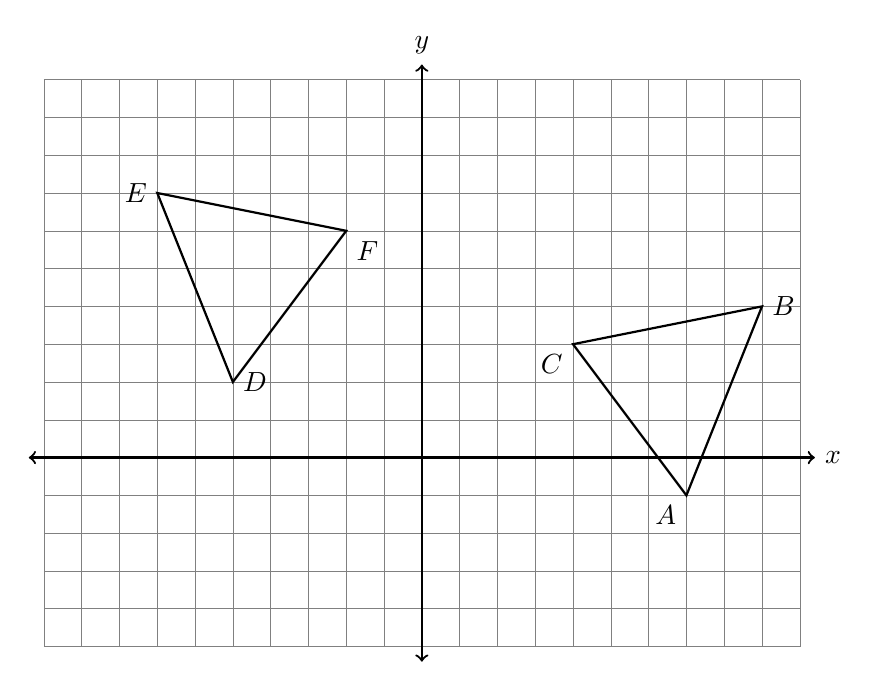
\begin{tikzpicture}[scale=.48]
      \draw [help lines] (-10,-5) grid (10,10);
      \draw [thick, <->] (-10.4,0) -- (10.4,0) node [right] {$x$};
      \draw [thick, <->] (0,-5.4)--(0,10.4) node [above] {$y$};
      \draw [thick]
        (7,-1) node[below left] {$A$}--
        (9,4) node[right] {$B$}--
        (4,3) node[below left] {$C$}--cycle;
      \draw [thick]
        (-5,2) node[right] {$D$}--
        (-7,7) node[left] {$E$}--
        (-2,6) node[below right] {$F$}--cycle;
    \end{tikzpicture}
  \end{flushright}

\item Reflect $\triangle ABC$ over the $y$-axis. Make a table of the coordinates and plot and label the image on the axes.
  \begin{flushright}
  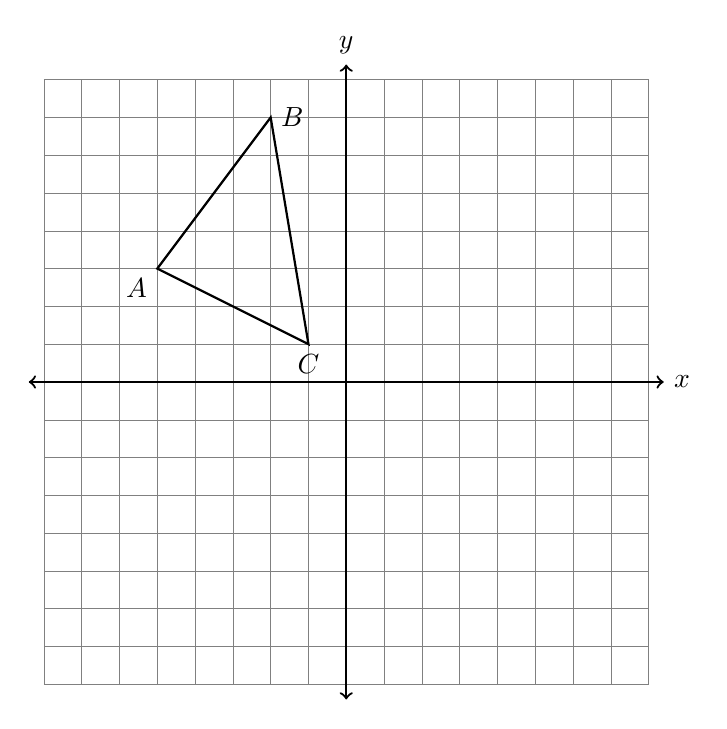
\begin{tikzpicture}[scale=.48]
    \draw [help lines] (-8,-8) grid (8,8);
    \draw [thick, <->] (-8.4,0) -- (8.4,0) node [right] {$x$};
    \draw [thick, <->] (0,-8.4)--(0,8.4) node [above] {$y$};  
    \draw [thick]
      (-5,3) node[below left] {$A$}--
      (-2,7) node[right] {$B$}--
      (-1,1) node[below] {$C$}--cycle;  
  \end{tikzpicture}
  \end{flushright}

\newpage
\item Rotate $\triangle ABC$ $90^\circ$ counterclockwise around the origin, yielding $\triangle A'B'C'$. Then translate it by $(x,y) \rightarrow (x+2, y+7)$. Make a table of the coordinates showing $\triangle ABC \rightarrow \triangle A'B'C' \rightarrow \triangle A''B''C''$ and plot and label the images on the axes.
  \begin{flushright}
      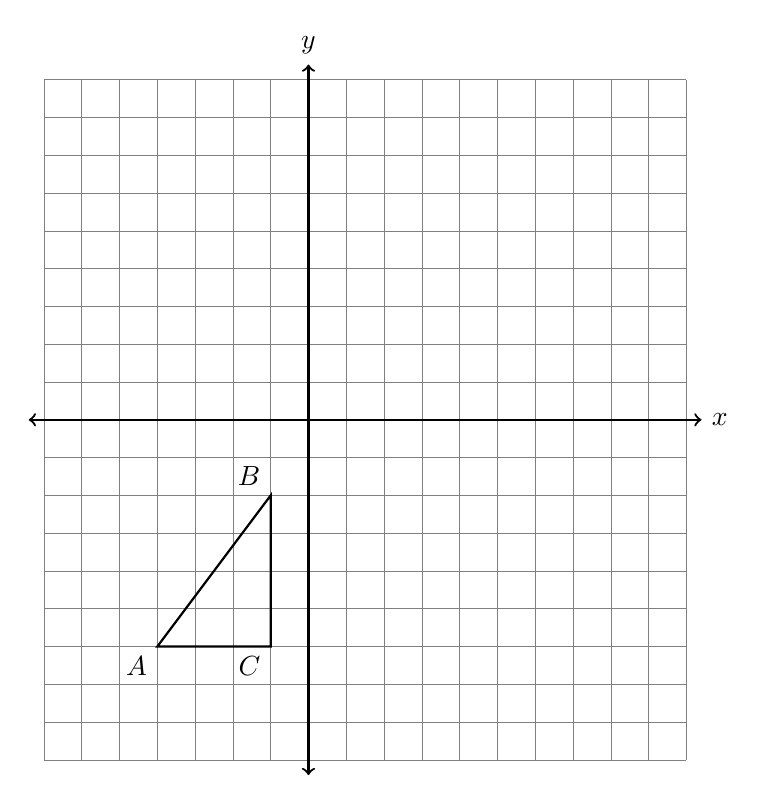
\begin{tikzpicture}[scale=.48]
      \draw [help lines] (-7,-9) grid (10,9);
      \draw [thick, <->] (-7.4,0) -- (10.4,0) node [right] {$x$};
      \draw [thick, <->] (0,-9.4)--(0,9.4) node [above] {$y$};  
      \draw [thick]
        (-4,-6) node[below left] {$A$}--
        (-1,-2) node[above left] {$B$}--
        (-1,-6) node[below left] {$C$}--cycle;  
    \end{tikzpicture}
  \end{flushright}

\item The $\triangle ABC$ is reflected across $l$ to yield $\triangle A'B'C'$. $AB=4x+4$, $A'B'=7x-8$, and $BC=5x+10$. Find the length $B'C'$. %\vspace{2cm}
  \begin{flushright}
  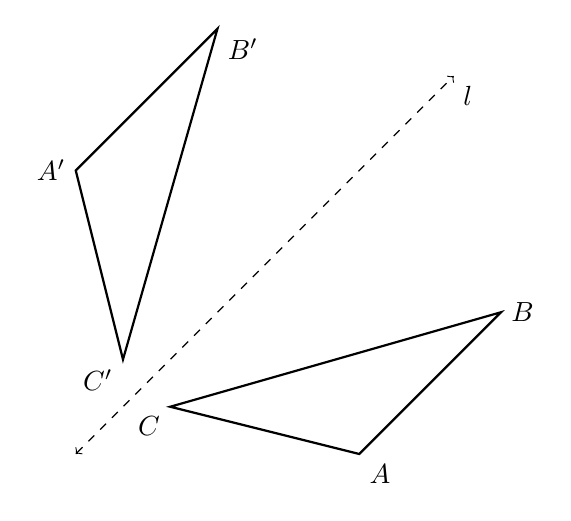
\begin{tikzpicture}[scale=.6]
    \draw [dashed, <->] (-1,-1)--(7,7) node[below right]{$l$};
    \draw [thick]
    (5,-1) node[below right] {$A$}--
    (8,2) node[right] {$B$}--
    (1,0) node[below left] {$C$}--cycle;
    \draw [thick]
    (-1,5) node[left] {$A'$}--
    (2,8) node[below right] {$B'$}--
    (0,1) node[below left] {$C'$}--cycle;
  \end{tikzpicture}
\end{flushright}

\newpage
\subsubsection*{Using the distance formula to prove an isosceles triangle}
\item In this problem use the following theorem (copy it at the bottom of the page after your calculations): \\*[0.25cm]
  \emph{A triangle is isosceles if and only two of its sides are congruent.}\\*[0.5cm]
  Shown below is triangle $ABC$, $A(-2,2)$, $B(4,5)$, and $C(1,-1)$. \\*[0.25cm]
  Prove it is an isosceles triangle by
  \begin{enumerate}
    \item finding the length of each of the three sides,
    \item stating which sides are congruent,
    \item copying the theorem as your conclusion, adding \emph{therefore $\triangle ABC$ is isosceles}.
  \end{enumerate}
  \begin{flushright} %4 quadrant regents grid
    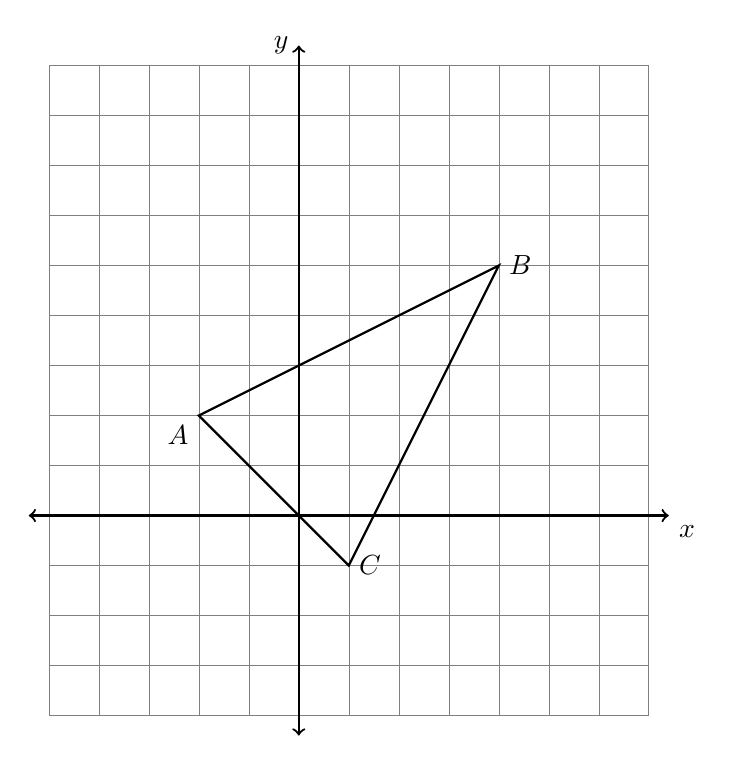
\begin{tikzpicture}[scale=.635]
      \draw [help lines] (-5,-4) grid (7,9);
      \draw [thick, <->] (-5.4,0) -- (7.4,0) node [below right] {$x$};
      \draw [thick, <->] (0,-4.4)--(0,9.4) node [left] {$y$};
      \draw [thick] (-2,2) node[below left] {$A$}--
      (4,5) node[right] {$B$}--
      (1,-1) node[right] {$C$}--cycle;
    \end{tikzpicture}
  \end{flushright}

\end{enumerate}
\end{document}